\subsection{Мера. Геометрическая вероятность}
\subsubsection{Мера Жордана}
Очевидно, что классическое определение вероятности не подходит для задач, где множество $\Omega$ является бесконечным. Например при игре в дартс можно говорить о бесконечном количестве точек на мишени, в которые мы можем попасть, следовательно о бесконечном количестве элементарных исходов. Однако даже интуитивно понятно, что при наличии некоторых вводных данных вполне возможно определить вероятность попадания в интересующую нас область.\\
Геометрическая вероятность позволяет нам решать такие задачи, но для полного её осознания нам потребуется понятие меры Лебега.\\
\begin{notice}На самом деле, полноценное изучение понятия меры требует отдельного курса. Здесь мы затронем лишь те утверждения, которые удобны и полезны нам (в упрощенном виде).
\end{notice}
\medskip
Для начала вспомним известную нам из курса матанализа меру Жордана.

\begin{definition}[Мера Жордана]
Пусть $\mathcal{P}$ -- множество всех многоугольных фигур (для наглядности можно взять фигуры на $\mathbb{R}^2$).

Мера Жордана (площадь в общем виде) -- это функция $\mu: \mathcal{P} \to \mathbb{R}$, которая удовлетворяет следующим четырём аксиомам:
\begin{enumerate}
    \item Для любого многоугольника $p \in \mathcal{P}$ верно, что $\mu(p) \ge 0$.
    
    \item Если $p_1, p_2 \in \mathcal{P}$ и $p_1 \cong$ (конгруэнтно) $p_2$ (то есть $p_1$ и $p_2$ совпадут при наложении), то $\mu(p_1) = \mu(p_2)$.
    
    \item Если $p_1, p_2 \in \mathcal{P}$ и  $p_1 \cap p_2 = \varnothing$, то
     $\mu(p_1 \cup p_2) = \mu(p_1) + \mu(p_2).$
    
    \item Для единичного квадрата $e \in \mathcal{P}$ (со стороной 1) выполняется $\mu(e) = 1$.
\end{enumerate}
\end{definition}


Пусть $\mathcal{P}$ -- множество всех многоугольников, для которых мера $\mu$ уже определена (удовлетворяет четырём аксиомам). Пусть $F$ -- произвольная ограниченная фигура на плоскости.

Рассмотрим два класса многоугольников:
\begin{itemize}
    \item все $p \in \mathcal{P}$, которые лежат внутри $F$ (то есть $p \subseteq F$);
    \item все $q \in \mathcal{P}$, которые содержат $F$ (то есть $F \subseteq q$).
\end{itemize}

\begin{definition}[Нижняя мера Жордана]
Нижняя мера Жордана (внутренняя) фигуры $F$ определяется как:
\[
\mu_*(F) = \sup_{\substack{p \in \mathcal{P} \\ p \subseteq F}} \mu(p).
\]
\end{definition}

\begin{definition}[Верхняя мера Жордана]
Верхняя мера Жордана (внешняя) фигуры $F$ определяется как:
\[
\mu^*(F) = \inf_{\substack{q \in \mathcal{P} \\ F \subseteq q}} \mu(q).
\]
\end{definition}

\begin{definition}[Измеримость по Жордану]
Фигура $F$ называется измеримой по Жордану (квадрируемой), если $\mu_*(F) = \mu^*(F)$. В этом случае число
\[
\mu(F) = \mu_*(F) = \mu^*(F)
\]
называется мерой Жордана (площадью) фигуры $F$.
\end{definition}


В матанализе эта мера используется для введения критерия интегрируемости и в качестве "фундамента" теории кратных интегралов. Нам же она нужна для проведения аналогии с мерой Лебега.

\subsubsection{Покрытие множества}

Наряду с верхней и нижней мерой Жордана существуют внешнее и внутреннее покрытия множеств. Грубо говоря, для нас это почти одно и то же, только теперь мы говорим не о произвольных фигурах, а о множествах

\begin{definition}[Внешнее покрытие множества]
Внешним покрытием множества $S$ называется такой набор множеств $\mathcal{A} = \{A_i\}_{i \in I}$, что
\[
S \subseteq \bigcup_{i \in I} A_i.
\]
\end{definition}

\begin{definition}[Внутреннее покрытие множества]
Внутренним покрытием множества $S$ называется такой набор множеств $\mathcal{A} = \{A_i\}_{i \in I}$, что
\[
\bigcup_{i \in I} A_i \subseteq S.
\]
\end{definition}

То есть мы как бы выбираем маленькие части-кусочки на множестве и говорим, что мы можем как полностью покрыть все множество некоторым числом таких "кусочков", так и поместить некоторое число кусочков полностью "внутрь" множества


%Картинка%
\begin{figure}[H]
    \centering
    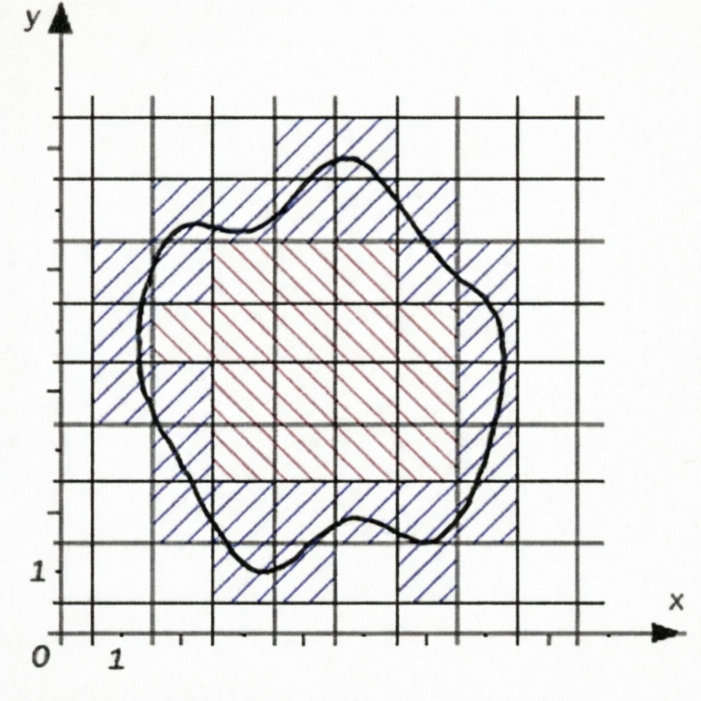
\includegraphics[width=0.5\textwidth]{images/quad.png}
    \caption{Иллюстрация внешнего и внутреннего покрытия множества точек, принаджлежащих фигуре}
    \label{fig:area_approximation}
\end{figure}

\subsubsection{Мера Лебега}

\begin{definition}[Внешняя мера Лебега]
Внешней мерой Лебега на $\mathbb{R}^n$ будем называть функцию $\mu^*: \mathcal{P}(\mathbb{R}^n) \to [0; +\infty]$, удовлетворяющей следующим свойствам:
\begin{itemize}
    \item $\mu^*([a_1; b_1] \times \ldots \times [a_n; b_n]) = \prod_{i=1}^{n} (b_i - a_i)$;
    \item Если $\mathcal{A}$ -- внешнее счётное покрытие множества $S$ многомерными прямоугольниками, то $\mu^*(S) = \inf_{\mathcal{A}} \sum_{i=1}^{\infty} \mu^*(A_i)$.
\end{itemize}
\end{definition}

\begin{definition}[Внутренняя мера Лебега]
Внутренней мерой Лебега на $\mathbb{R}^n$ будем называть функцию $\mu_*: \mathcal{P}(\mathbb{R}^n) \to [0; +\infty]$, удовлетворяющей следующим свойствам:
\begin{itemize}
    \item $\mu_*([a_1; b_1] \times \ldots \times [a_n; b_n]) = \prod_{i=1}^{n} (b_i - a_i)$;
    \item Если $\mathcal{A}$ -- внутреннее счётное покрытие множества $S$ многомерными прямоугольниками, то $\mu_*(S) = \sup_{\mathcal{A}} \sum_{i=1}^{\infty} \mu_*(A_i)$.
\end{itemize}
\end{definition}

\begin{definition}[Измеримость по Лебегу и мера Лебега]
Множество $S \subset \mathbb{R}^n$ является \textbf{измеримым по Лебегу}, если его внешняя мера совпадает с внутренней мерой.

\textbf{Мерой Лебега} измеримого множества $S$ -- его внешняя мера. Меру Лебега будем обозначать как $\mu$.
\end{definition}


Выделим основные свойства меры Лебега:

\begin{notice}
\begin{enumerate}
    \item \textbf{Монотонность:} $S_1 \subseteq S_2 \Rightarrow \mu(S_1) \leqslant \mu(S_2)$;
    \item \textbf{Счётная полуаддитивность:} $S = \bigcup_{i=1}^{\infty} S_i \Rightarrow \mu(S) \leqslant \sum_{i=1}^{\infty} \mu(S_i)$;
    \item \textbf{Счётная аддитивность:} $S = \bigsqcup_{i=1}^{\infty} S_i \Rightarrow \mu(S) = \sum_{i=1}^{\infty} \mu(S_i)$.
\end{enumerate}
\end{notice}

Мера Лебега на $\mathbb{R}^n$ является обобщением понятий длины отрезка, площади фигуры и объёма тела на произвольное $n$-мерное евклидово пространство.

Наконец, определим геометрическую вероятность.

\begin{definition}[Геометрическая вероятность]
Геометрической вероятностью события $A$ называется отношение мер Лебега множества $A$ и множества $\Omega$:
\[
\mathbb{P}(A) = \frac{\mu(A)}{\mu(\Omega)}.
\]
\end{definition}